\documentclass[11pt]{article}
%\include{amsfonts}
%\usepackage{amssymb,amsmath,latexsym,epsfig,euscript}
\usepackage{amssymb}
\usepackage{enumitem}
\usepackage{amsmath}
\usepackage{multicol}

\usepackage{bm}


%
\def\d{\displaystyle}
%
\usepackage[heightrounded]{geometry}
\geometry{top=2cm,bottom=2cm,left=2cm,right=2cm}
\parindent=0pt

\usepackage{graphicx}
\graphicspath{ {../images} }

\usepackage{listings}
\lstset{
  basicstyle=\ttfamily,
  columns=fullflexible,
}

\usepackage{url}
\usepackage{multicol}
\usepackage{dsfont}

% Bold symbols for vectors and matrices
\newcommand{\xstar}{\bm{x}^{\star}}
\newcommand{\alphab}{\bm{\alpha}}
\newcommand{\ab}{\bm{a}}
\newcommand{\bb}{\bm{b}}
\newcommand{\cb}{\bm{c}}
\newcommand{\db}{\bm{d}}
\newcommand{\eb}{\bm{e}}
\newcommand{\gb}{\bm{g}}
\newcommand{\mb}{\bm{m}}
\newcommand{\pb}{\bm{p}}
\newcommand{\qb}{\bm{q}}
\newcommand{\rb}{\bm{r}}
\newcommand{\ssb}{\bm{s}}
\newcommand{\ub}{\bm{u}}
\newcommand{\vb}{\bm{v}}
\newcommand{\wb}{\bm{w}}
\newcommand{\xb}{\bm{x}}
\newcommand{\yb}{\bm{y}}
\newcommand{\zb}{\bm{z}}

\newcommand{\Ab}{\bm{A}}
\newcommand{\Bb}{\bm{B}}
\newcommand{\Cb}{\bm{C}}
\newcommand{\Db}{\bm{D}}
\newcommand{\Eb}{\bm{E}}
\newcommand{\Fb}{\bm{F}}
\newcommand{\Gb}{\bm{G}}
\newcommand{\Hb}{\bm{H}}
\newcommand{\Ib}{\bm{I}}
\newcommand{\Id}{\bm{I}}
\newcommand{\Kb}{\bm{K}}
\newcommand{\Lb}{\bm{L}}
\newcommand{\Mb}{\bm{M}}
\newcommand{\Pb}{\bm{P}}
\newcommand{\Qb}{\bm{Q}}
\newcommand{\Rb}{\bm{R}}
\newcommand{\Sb}{\bm{S}}
\newcommand{\Tb}{\bm{T}}
\newcommand{\Ub}{\bm{U}}
\newcommand{\Vb}{\bm{V}}
\newcommand{\Wb}{\bm{W}}
\newcommand{\Xb}{\bm{X}}
\newcommand{\Yb}{\bm{Y}}
\newcommand{\Zb}{\bm{Z}}
\newcommand{\Lambdab}{\bm{\Lambda}}
\newcommand{\cero}{\bm{0}}

% Rings and fields
\newcommand{\A}{\mathbb{A}}
\newcommand{\Z}{\mathbb{Z}}
\newcommand{\Q}{\mathbb{Q}}
\newcommand{\C}{\mathbb{C}}
\newcommand{\R}{\mathbb{R}}
\newcommand{\K}{\mathbb{K}}
\newcommand{\N}{\mathbb{N}}

\newcommand{\borel}{{\mathcal B}}
\newcommand{\pmom}{{\rho_{\text{mom}}}}
\newcommand{\MX}{{\mathcal{M}(X)}}


% Inner product
\newcommand{\innerl}[2]{\langle #1, #2 \rangle}
\newcommand{\inner}[2]{#1 \boldsymbol{\cdot} #2}
\newcommand{\innerTrace}[2]{#1 \bullet #2}

% Symmetric and positive definite matrices
\newcommand{\Splusplusn}{{\mathcal S_{++}^n}}
\newcommand{\Splusn}{{\mathcal S_+^n}}
\newcommand{\Splus}{{\mathcal S_+}}
\newcommand{\Sym}{{\mathcal S}}
\newcommand{\Symn}{{\mathcal S^n}}

% Cones
\newcommand\CC{\mathcal{C}}
\DeclareMathOperator{\cone}{cono}
\DeclareMathOperator{\conv}{conv}
\DeclareMathOperator{\supp}{supp}


% Spectrahedron
\newcommand{\eLL}{{\mathcal L}}

% Matrices and vectors over R or C
\newcommand{\Rnn}{\R^{n\times n}}
\newcommand{\Cnn}{\C^{n\times n}}
\newcommand{\Rn}{\R^{n}}
\newcommand{\Rm}{\R^{m}}


% Math operators
\DeclareMathOperator{\Tr}{Tr}
\DeclareMathOperator{\tr}{Tr}
\DeclareMathOperator{\interior}{int}
\DeclareMathOperator{\rank}{rank}
\DeclareMathOperator{\diag}{diag}

\newcommand\one{\mathds{1}} 


\begin{document}

\begin{center}

{\small Facultad de Ciencias Exactas
y Naturales -- Universidad de Buenos Aires } \vskip 1cm

\textbf{{\large Optimización Semidefinida} - Segundo Cuatrimestre 2021}

\medskip\textbf{Pr\'actica 3 - Aplicaciones SDP}
\end{center}

\medskip

\textbf{Para entregar:} entregar un ejercicio a elección entre los marcados ($\diamondsuit$).

\vspace{0.5cm}

\noindent \textbf{Max-cut}

\begin{enumerate}

\item En los siguientes ejemplos, se considera que el costo de las aristas que aparecen dibujadas en el grafo es 1, y que el costo de las aristas que no aparecen es 0. Llamamos $K$ al conjunto de puntos azules dentro de la región marcada.

\begin{center}
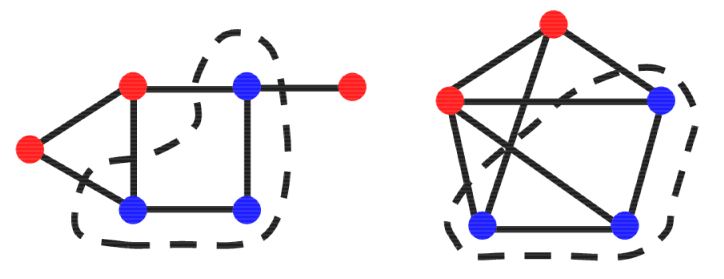
\includegraphics[scale=2]{cut_example_2.png}
\end{center}

Para cada uno de los ejemplos:

\begin{enumerate}
\item Calcular a mano el costo de los cortes marcados.
\item Construir la matriz $\Qb$ de costos.
\item Numerar los nodos de 1 a $n$ y representar el corte marcado como un vector $\xb \in \{-1, 1\}^n$, donde $x_i=1$ sii $i$ pertenece a $K$
\item Construir una matriz $\Cb$ tal que el costo de un corte determinado por un vector $\xb$ sea $\xb^T \Cb \xb$.
\item Para el corte dado, verificar las cuentas en Python.
\item Buscar, por prueba y error, algún corte que tenga mayor costo que el corte dado.
\end{enumerate}

\item Implementar un programa que reciba una matriz $\Qb$ de costos y calcule el corte de mayor costo probando todos los cortes posibles. Aplicar el programa a los ejemplos anteriores y verificar si el corte coincide con el corte del ejemplo o con el mejor corte que haya encontrado en el último punto.

\item Utilizar el programa anterior para hallar el corte de mayor costo en el siguiente ejemplo.
\begin{center}
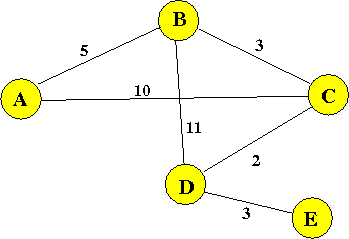
\includegraphics[scale=2]{maxcut-netw.png}
\end{center}

\item \textbf{Programación lineal.}
\begin{enumerate}
\item Verificar que el siguiente problema de programación entera
\begin{alignat*}{2}
  & \text{maximizar: } &  &  \sum_{1 \le i, j, \le n} w_{ij} z_{ij}\\
  & \text{sujeto a: }&  \quad & z_{ij} \le x_i + x_j,  \forall \  1 \le i,j, \le n \\
  &&& z_{ij} \le 2 - (x_i + x_j), \forall \ 1 \le i,j, \le n \\
   &&& x_i, z_{ij} \in \{0, 1\} \forall \  1 \le i,j, \le n
\end{alignat*}
es una formulación del problema max-cut tomando para un subconjunto $K$ de nodos, $x_i = 1$ sii $i \in K$ y $z_{ij} = 1$ sii $(i,j) \in \delta(K)$.

\item Para convertirlo en una problema de programación lineal podemos relajar la restricciones $x_i, z_{ij} \in \{0, 1\} \forall i, j,$ a $x_i, z_{ij} \in [0,1] \forall i, j$. ¿Considera que esta relajación es una buena aproximación al problema original?

\item (*) Utilizando que en un conjunto cualquiera de tres nodos del grafo, no pueden estar las tres aristas en el corte, formular una mejor relajación como problema de programación lineal.

\item (*) Calcular en los ejemplos de los ejercicios anteriores el cociente entre el valor óptimo de la relajación y el valor óptimo del problema original.


\end{enumerate}

\item Implementar en Mosek la relajación SDP del problema max-cut. Aplicar el programa en los ejemplos anteriores y comparar el costo óptimo del problema original con el valor óptimo del problema relajado.

\item ($\diamondsuit$) Demostrar que la solución óptima del problema SDP
\begin{alignat*}{2}
  & \text{minimizar: } &  &  \Tr(\Lambda)\\
  & \text{sujeto a: }&  \quad & \Cb \preceq \Lambda  \\
  &&& \Lambda \text{ diagonal}
\end{alignat*}
es una cota superior del costo óptimo $\xb^T \Cb \xb$, $\xb \in \{-1, +1\}^n$, del problema max-cut.

Verificar que dicho problema es el problema dual de la relajación SDP vista en clase del problema SDP.

Implementar este problema en Mosek y calcular el óptimo para el caso de un pentágono.

\item Implementar un programa que dado $n \in \N$, devuelva una matriz simétrica cuyas entradas sean números aleatorios entre 0 y 1.
Sugerencia: utilizar el comando \texttt{np.random.rand}.

\item Comparar el costo óptimo del problema original con el valor óptimo del problema relajado para matrices aleatorias de tamaño 5, 10 y 15.

\item (*) Dadas $n$ variables aleatorias $r_1, \dots, r_n$ con distribución normal (gaussiana) $N(0,1)$, probar que el vector
$$
\vb = \frac{(r_1, \dots, r_n)}{\|(r_1, \dots, r_n)\|_2}
$$
es un vector en la esfera unitaria con distribución uniforme sobre la esfera.

Sugerencia: probar que la densidad conjunta de $(r_1, \dots, r_n)$ solo depende de la norma del vector.

\item Implementar en Python un programa que genere un vector aleatorio en la esfera unitaria de dimensión $n$, con distribución uniforme sobre la misma.

\item Implementar un programa que dado un vector unitario $\rb \in \Rn$ y una matriz $\Pb \in \Rn$ cuyas columnas son vectores unitarios, devuelva un vector $\xb \in \{-1, +1\}^n$ con $x_i = +1$ sii $\inner{\rb}{\pb_i} > 0$, con $\pb_i$ la $i$-ésima columna de $\Pb$.

\item Implementar un programa que a partir de la matrix $\Xb$ que se obtiene como solución óptima de la relajación SDP del problema max-cut con valor óptimo $s$, calcule un vector $\xb \in \{-1, +1\}^n$ tal que el corte asociado a dicho vector satisfaga
    $$
    w(\delta(\xb)) \ge 0.878 s
    $$

\item En todos los ejemplos de los ejercicios anteriores, calcular la razón entre las soluciones óptimas del problema maxcut original y la relajación SDP.

\item Calcular la razón entre las soluciones óptimas del problema maxcut original y la relajación SDP para el pentágono
\begin{center}
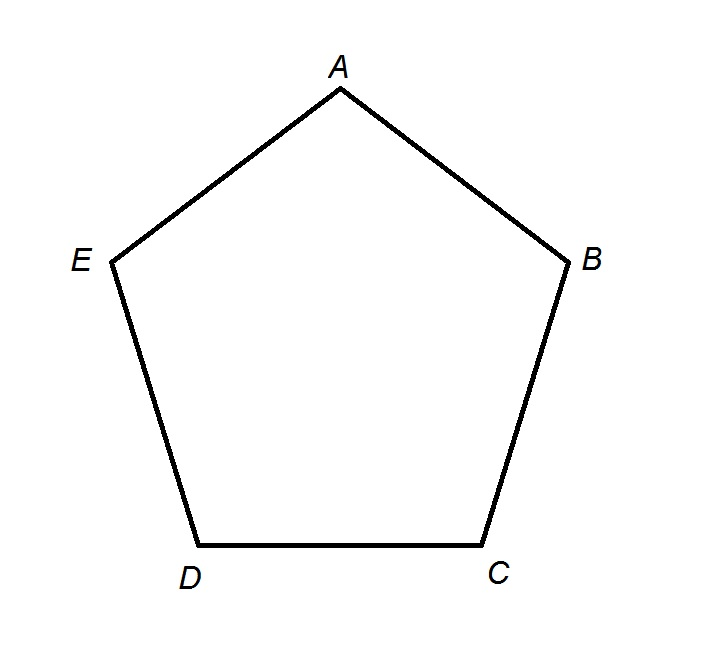
\includegraphics[scale=.3]{maxcut-Pentagon.jpg}
\end{center}
tomando costo 1 para los lados del pentágono y costo 0 para las demás aristas.

\end{enumerate}


\noindent \textbf{Teoría de control}

\begin{enumerate}[resume]

\item Para la matriz
$$
\Pb = \begin{pmatrix} 3 & x \\ x & 3 \end{pmatrix},
$$
\begin{enumerate}
\item calcular los autovalores en función de $x$.
\item resolver a mano el problema SDP
\begin{alignat*}{2}
  & \text{minimizar: } & & x_{11} \\
   & \text{sujeto a: } & \quad & \Pb \succ 0, \\
\end{alignat*}
\item resolver a mano el problema SDP
\begin{alignat*}{2}
  & \text{minimizar: } & & x_{11} \\
   & \text{sujeto a: } & \quad & \Pb \succeq \Ib, \\
\end{alignat*}
\item resolver a mano el problema SDP
\begin{alignat*}{2}
  & \text{minimizar: } & \quad & \eta \\
   & \text{sujeto a: } & & \Ib \preceq \Pb \preceq \eta \Ib, \\
\end{alignat*}
\end{enumerate}

\item ($\diamondsuit$) Implementar un programa que reciba una matriz $\Ab \in \R^{n \times n}$ y resuelva el problema SDP
\begin{alignat*}{2}
  & \text{minimizar: } & & p_{00} \\
   & \text{sujeto a: } & \quad & \Ab^T \Pb \Ab - \Pb \succ 0, \\
   &&& \Pb - \Ib \succeq 0, \\
\end{alignat*}

\item ($\diamondsuit$) Implementar un programa que reciba una matriz $\Ab \in \R^{2 \times 2}$ y resuelva el problema SDP
\begin{alignat*}{2}
  & \text{minimizar: } & & \eta \\
   & \text{sujeto a: } & \quad & \Ab^T \Pb \Ab - \Pb \succ 0, \\
   &&& \Pb - \Ib \succeq 0, \\
   &&& \eta \Ib - \Pb \succeq 0
\end{alignat*}

\item Para las siguientes matrices $\Ab \in \R^{n \times n}$, $\Bb \in \R^{n \times m}$, determinar si existe $\Kb \in \R^{m \times n}$ tal que $\rho(\Ab + \Bb \Kb) \le 1$.
\begin{enumerate}
\item $\Ab = \begin{pmatrix} 10 & 0 \\ 0 & 0.5 \end{pmatrix}$, $\Bb = \begin{pmatrix} 2 & 3 \\ 1 & 4 \end{pmatrix}$.
\item $\Ab = \begin{pmatrix} 10 & 0 \\ 0 & 0.5 \end{pmatrix}$, $\Bb = \begin{pmatrix} 2 & 0 \\ 1 & 0 \end{pmatrix}$.
\item $\Ab = \begin{pmatrix} 10 & 0 \\ 0 & 0.5 \end{pmatrix}$, $\Bb = \begin{pmatrix} 2 & 1 \\ 0 & 0 \end{pmatrix}$.
\end{enumerate}

Intentar resolver los problemas analíticamente y verificar los resultados con Mosek.

\item Un sistema de la forma
$$
\xb[k+1] = \Ab\xb[k] + \Bb\ub[k], \quad \xb[0] = \xb_0,
$$
tiene un \emph{modo no estabilizable} si la matriz $\Ab$ tiene un autovector a izquierda $\wb$ tal que
$$
\wb^T \Ab = \lambda \wb^T, \quad \wb^T \Bb = 0 \quad \text{ y } \quad |\lambda| \ge 1
$$

\begin{itemize}
\item Probar que en ese caso, el problema SDP no es factible.
\item Interpretar el resultado en término de los autovalores de $\Ab + \Bb \Kb$.
\end{itemize}

\item (Estabilización con retroalimentación de salida.) Considerar el siguiente sistema de control para matrices $\Ab \in \Rnn$, $\Bb \in \R^{n \times k}$ y $\Cb \in \R^{k \times r}$:
\begin{center}
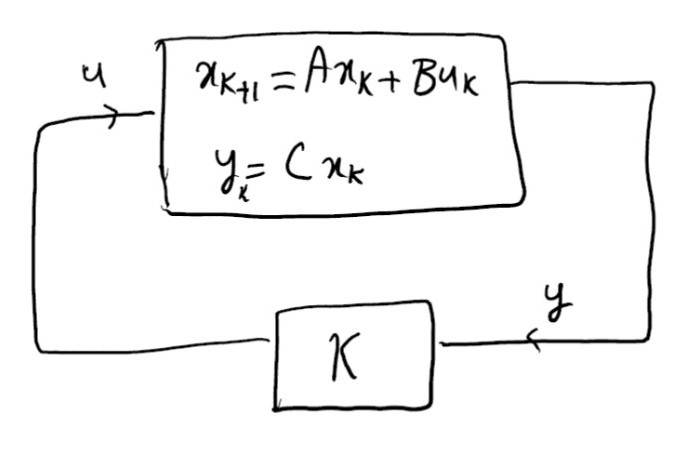
\includegraphics[scale=.5]{control-loop-output.jpg}
\end{center}

\begin{enumerate}
\item Verificar que la estabilidad del sistema es equivalente a la existencia de una matriz $\Kb \in \R^{k \times r}$ tal que $\rho(A + BKC ) < 1$.
\item Plantear este problema como un problema SDP. Nota: la existencia de dicho problema SDP ¡es un problema abierto!
\end{enumerate}
\end{enumerate}





Los ejercicios marcados (*) son optativos y pueden involucrar temas no vistos en la materia.
\end{document}
